\documentclass{mimosis}

\usepackage{metalogo}

%%%%%%%%%%%%%%%%%%%%%%%%%%%%%%%%%%%%%%%%%%%%%%%%%%%%%%%%%%%%%%%%%%%%%%%%
% Some of my favourite personal adjustments
%%%%%%%%%%%%%%%%%%%%%%%%%%%%%%%%%%%%%%%%%%%%%%%%%%%%%%%%%%%%%%%%%%%%%%%%
%
% These are the adjustments that I consider necessary for typesetting
% a nice thesis. However, they are *not* included in the template, as
% I do not want to force you to use them.

% This ensures that I am able to typeset bold font in table while still aligning the numbers
% correctly.
\usepackage{etoolbox}

\usepackage[binary-units=true]{siunitx}
\DeclareSIUnit\px{px}

\sisetup{%
  detect-all           = true,
  detect-family        = true,
  detect-mode          = true,
  detect-shape         = true,
  detect-weight        = true,
  detect-inline-weight = math,
}

%%%%%%%%%%%%%%%%%%%%%%%%%%%%%%%%%%%%%%%%%%%%%%%%%%%%%%%%%%%%%%%%%%%%%%%%
% Hyperlinks & bookmarks
%%%%%%%%%%%%%%%%%%%%%%%%%%%%%%%%%%%%%%%%%%%%%%%%%%%%%%%%%%%%%%%%%%%%%%%%

\usepackage[%
  colorlinks = true,
  citecolor  = Green,
  linkcolor  = RoyalBlue,
  urlcolor   = RoyalBlue,
  unicode,
  ]{hyperref}

\usepackage{bookmark}

%%%%%%%%%%%%%%%%%%%%%%%%%%%%%%%%%%%%%%%%%%%%%%%%%%%%%%%%%%%%%%%%%%%%%%%%
% Bibliography
%%%%%%%%%%%%%%%%%%%%%%%%%%%%%%%%%%%%%%%%%%%%%%%%%%%%%%%%%%%%%%%%%%%%%%%%
%
% I like the bibliography to be extremely plain, showing only a numeric
% identifier and citing everything in simple brackets. The first names,
% if present, will be initialized. DOIs and URLs will be preserved.

\usepackage[%
  autocite     = plain,
  backend      = biber,
  doi          = true,
  url          = true,
  giveninits   = true,
  hyperref     = true,
  maxbibnames  = 99,
  maxcitenames = 99,
  sortcites    = true,
  style        = numeric,
  ]{biblatex}

%%%%%%%%%%%%%%%%%%%%%%%%%%%%%%%%%%%%%%%%%%%%%%%%%%%%%%%%%%%%%%%%%%%%%%%%
% Some adjustments to make the bibliography more clean
%%%%%%%%%%%%%%%%%%%%%%%%%%%%%%%%%%%%%%%%%%%%%%%%%%%%%%%%%%%%%%%%%%%%%%%%
%
% The subsequent commands do the following:
%  - Removing the month field from the bibliography
%  - Fixing the Oxford commma
%  - Suppress the "in" for journal articles
%  - Remove the parentheses of the year in an article
%  - Delimit volume and issue of an article by a colon ":" instead of
%    a dot ""
%  - Use commas to separate the location of publishers from their name
%  - Remove the abbreviation for technical reports
%  - Display the label of bibliographic entries without brackets in the
%    bibliography
%  - Ensure that DOIs are followed by a non-breakable space
%  - Use hair spaces between initials of authors
%  - Make the font size of citations smaller
%  - Fixing ordinal numbers (1st, 2nd, 3rd, and so) on by using
%    superscripts

% Remove the month field from the bibliography. It does not serve a good
% purpose, I guess. And often, it cannot be used because the journals
% have some crazy issue policies.
\AtEveryBibitem{\clearfield{month}}
\AtEveryCitekey{\clearfield{month}}

% Fixing the Oxford comma. Not sure whether this is the proper solution.
% More information is available under [1] and [2].
%
% [1] http://tex.stackexchange.com/questions/97712/biblatex-apa-style-is-missing-a-comma-in-the-references-why
% [2] http://tex.stackexchange.com/questions/44048/use-et-al-in-biblatex-custom-style
%
\AtBeginBibliography{%
  \renewcommand*{\finalnamedelim}{%
    \ifthenelse{\value{listcount} > 2}{%
      \addcomma
      \addspace
      \bibstring{and}%
    }{%
      \addspace
      \bibstring{and}%
    }
  }
}

% Suppress "in" for journal articles. This is unnecessary in my opinion
% because the journal title is typeset in italics anyway.
\renewbibmacro{in:}{%
  \ifentrytype{article}
  {%
  }%
  % else
  {%
    \printtext{\bibstring{in}\intitlepunct}%
  }%
}

% Remove the parentheses for the year in an article. This removes a lot
% of undesired parentheses in the bibliography, thereby improving the
% readability. Moreover, it makes the look of the bibliography more
% consistent.
\renewbibmacro*{issue+date}{%
  \setunit{\addcomma\space}
    \iffieldundef{issue}
      {\usebibmacro{date}}
      {\printfield{issue}%
       \setunit*{\addspace}%
       \usebibmacro{date}}%
  \newunit}

% Delimit the volume and the number of an article by a colon instead of
% by a dot, which I consider to be more readable.
\renewbibmacro*{volume+number+eid}{%
  \printfield{volume}%
  \setunit*{\addcolon}%
  \printfield{number}%
  \setunit{\addcomma\space}%
  \printfield{eid}%
}

% Do not use a colon for the publisher location. Instead, connect
% publisher, location, and date via commas.
\renewbibmacro*{publisher+location+date}{%
  \printlist{publisher}%
  \setunit*{\addcomma\space}%
  \printlist{location}%
  \setunit*{\addcomma\space}%
  \usebibmacro{date}%
  \newunit%
}

% Ditto for other entry types.
\renewbibmacro*{organization+location+date}{%
  \printlist{location}%
  \setunit*{\addcomma\space}%
  \printlist{organization}%
  \setunit*{\addcomma\space}%
  \usebibmacro{date}%
  \newunit%
}

% Display the label of a bibliographic entry in bare style, without any
% brackets. I like this more than the default.
%
% Note that this is *really* the proper and official way of doing this.
\DeclareFieldFormat{labelnumberwidth}{#1\adddot}

% Ensure that DOIs are followed by a non-breakable space.
\DeclareFieldFormat{doi}{%
  \mkbibacro{DOI}\addcolon\addnbspace
    \ifhyperref
      {\href{http://dx.doi.org/#1}{\nolinkurl{#1}}}
      %
      {\nolinkurl{#1}}
}

% Use proper hair spaces between initials as suggested by Bringhurst and
% others.
\renewcommand*\bibinitdelim {\addnbthinspace}
\renewcommand*\bibnamedelima{\addnbthinspace}
\renewcommand*\bibnamedelimb{\addnbthinspace}
\renewcommand*\bibnamedelimi{\addnbthinspace}

% Make the font size of citations smaller. Depending on your selected
% font, you might not need this.
\renewcommand*{\citesetup}{%
  \biburlsetup
  \small
}

\DeclareLanguageMapping{english}{english-mimosis}

\addbibresource{Thesis.bib}

%%%%%%%%%%%%%%%%%%%%%%%%%%%%%%%%%%%%%%%%%%%%%%%%%%%%%%%%%%%%%%%%%%%%%%%%
% Fonts
%%%%%%%%%%%%%%%%%%%%%%%%%%%%%%%%%%%%%%%%%%%%%%%%%%%%%%%%%%%%%%%%%%%%%%%%

\ifxetexorluatex
  \setmainfont{Minion Pro}
\else
  \usepackage[lf]{ebgaramond}
  \usepackage[oldstyle,scale=0.7]{sourcecodepro}
  \singlespacing
\fi

\renewcommand{\th}{\textsuperscript{\textup{th}}\xspace}

\newacronym[description={Principal component analysis}]{PCA}{PCA}{principal component analysis}
\newacronym                                            {SNF}{SNF}{Smith normal form}
\newacronym[description={Topological data analysis}]   {TDA}{TDA}{topological data analysis}

\newglossaryentry{LaTeX}{%
  name        = {\LaTeX},
  description = {A document preparation system},
  sort        = {LaTeX},
}

\newglossaryentry{Real numbers}{%
  name        = {$\real$},
  description = {The set of real numbers},
  sort        = {Real numbers},
}

\makeindex
\makeglossaries

%%%%%%%%%%%%%%%%%%%%%%%%%%%%%%%%%%%%%%%%%%%%%%%%%%%%%%%%%%%%%%%%%%%%%%%%
% Incipit
%%%%%%%%%%%%%%%%%%%%%%%%%%%%%%%%%%%%%%%%%%%%%%%%%%%%%%%%%%%%%%%%%%%%%%%%

\title{Object Detection in Manufacturing Industry}
\subtitle{\textsc{Master's thesis}}
\author{Hai Duong Tran}

\begin{document}

\frontmatter
  \begin{titlepage}

  \vspace*{1.5cm}
  \makeatletter

  \begin{center}
    \begin{LARGE}
        \textsc{Masaryk University}
    \end{LARGE}\\
    \begin{Large}
        \textsc{Faculty of Informatics}
    \end{Large}\\[1cm]
    
\includegraphics[width=4cm, height=4cm] {fi_logo.pdf}\\[2cm]
    \begin{Huge}
      \@title
    \end{Huge}\\[1.25cm]
    %
    \begin{Large}
      \@subtitle
    \end{Large}\\[1.5cm]
    \begin{LARGE}
    %
    \@author
    \end{LARGE}
    \vfill
    {\hfill\large Brno 2020}
  \end{center}
  \makeatother
\end{titlepage}

\newpage
\null
\thispagestyle{empty}
\newpage

  \chapter*{Declaration}

\noindent
Hereby I declare, that this paper is my original authorial work, which I
have worked out by my own. All sources, references and literature used or
excerpted during elaboration of this work are properly cited and listed in
complete reference to the due source.
\vfill
\textbf{Advisor:} doc. RNDr. Pavel Matula, Ph.D.
  \chapter*{Acknowledgements}
\noindent
Lorem ipsum dolor sit amet, consectetuer adipiscing elit. Temporibus autem quibusdam et aut officiis debitis aut rerum necessitatibus saepe eveniet ut et voluptates repudiandae sint et molestiae non recusandae. Proin in tellus sit amet nibh dignissim sagittis. Aliquam id dolor. Fusce dui leo, imperdiet in, aliquam sit amet, feugiat eu, orci. Sed vel lectus. Donec odio tempus molestie, porttitor ut, iaculis quis, sem. Nullam faucibus mi quis velit. Quisque porta. Integer pellentesque quam vel velit. Cum sociis natoque penatibus et magnis dis parturient montes, nascetur ridiculus mus.
  \chapter*{Abstract}
\noindent
This work is concerned with object detection in images based on state-of-the-art
deep neural networks. The thesis is a result of a collaboration with
company SANEZOO EUROPE that provided image datasets. The work introduces
selected object detection models that were further evaluated according to
appropriate metrics on provided datasets. For future evaluations of the models
on an arbitrary datasets, we implemented a simple benchmarking tool that
can be controlled via web user interface.

\section*{Keywords}
\noindent
SANEZOO EUROPE, image processing, visual recognition, object detection, deep
learning, machine learning, neural networks, benchmarking

  \tableofcontents

\mainmatter

  %%%%%%%%%%%%%%%%%%%%%%%%%%%%%%%%%%%%%%%%%%%%%%%%%%%%%%%%%%%%%%%%%%%%%%%%
\chapter{Introduction}
%%%%%%%%%%%%%%%%%%%%%%%%%%%%%%%%%%%%%%%%%%%%%%%%%%%%%%%%%%%%%%%%%%%%%%%%

In the era of Industry 4.0, companies exploit modern technology to optimize traditional manufacturing and industrial processes. As human labor is expensive, companies search for new ways to minimize human assistance. Eyesight is one of the senses that could not be replaced easily for a long time. However, with recent advances in the field of computer vision, some human tasks can be done by robots that consist of camera systems that allow robots to perceive their surroundings. 

In 2015 scientists from Microsoft Research team proposed a deep learning model that surpassed human-level accuracy on a visual recognition task on the ImageNet 2012 classification dataset \cite{surp2015}. Since then, even better models were proposed \cite{resnet, efficientnet}. These high-performing image recognition models became the backbone of state-of-the-art object detection models, which are the key component of machine perception.

There are many areas where machine perception can be useful in industry. For instance, the models can be trained to detect faulty products soon enough to take corrective actions to ensure the products' quality. It is also a vital part of robotic arms that can carry out non-trivial tasks such as picking, sorting, and packing items. Another example of use can be observed in autonomous delivery navigation robots that can pick up trays of objects and move them around in a large warehouse~\cite{bmw}. 
  %%%%%%%%%%%%%%%%%%%%%%%%%%%%%%%%%%%%%%%%%%%%%%%%%%%%%%%%%%%%%%%%%%%%%%%%
\chapter{Deep Learning}\label{deep_learning_chapter}
%%%%%%%%%%%%%%%%%%%%%%%%%%%%%%%%%%%%%%%%%%%%%%%%%%%%%%%%%%%%%%%%%%%%%%%%

% Neural networks since 60s
% Deep learning since 2006
% Definition
  % Multiple layers
  % Based on ANN
% Impact

In this chapter, we will briefly introduce some of the relevant topics of deep learning to the reader. We assume previous knowledge of the basics of machine learning and artificial neural networks (ANNs). All concepts in this chapter are very well described in the book written by the pioneers of deep learning, Ian Goodfellow, Yoshua Bengio, and Aaron Courville \cite{Goodfellow-et-al-2016}. 

The history of ANNs can be dated back to the 1940s \cite{McCulloch_1943}. However, only since 2006, deep architectures of ANN have become a trendy area of machine learning research \cite{DBLP:journals/corr/Schmidhuber14}. That year, Hinton et al. introduced unsupervised pre-training of deep feedforward neural networks. Using this method on a deep belief network \cite{DBN}, the model achieved 1.2\% error rate on the MNIST classification dataset \cite{mnist}. This exceptional result drew attention to deep belief networks. The historical development of artificial neural networks and deep learning is nicely overviewed in a journal article by another important figure in the field Juergen Schmidhuber 
\cite{DBLP:journals/corr/Schmidhuber14}.

\section{Definition}
Firstly, let us define the field of deep learning. Many of closely related definitions are summarized in \cite{mic_definitions}. We cite the one that best suits the nature of this work.  
    
\theoremstyle{definition}
\newtheorem*{definition}{Definition}
\begin{definition}\todo{Upravit. Doslovna citace. Pouziti definition bloku neni konzistentni s dalsimi definicemi.}
A class of machine learning techniques that exploit \textbf{many} layers of non-linear information processing for supervised or unsupervised feature extraction and transformation, and for pattern analysis and classification.
\end{definition}

In our case, the deep learning technique will be used for object detection, which also consists of the classification task. The selected object detection models are deep architectures of \textbf{convolutional neural network (CNN)}, which are particularly effective for image processing tasks. In the coming section, we will briefly describe the foundations of CNNs. 

\section{Convolutional Neural Network}
Deep neural networks are organized into multiple layers, which are typically sequentially ordered. In the following subsections, we will describe layers that we can find in CNNs.

\subsection{Fully-connected Layer}
The most basic layer is \textbf{fully-connected layer} (also known as \textbf{linear} or \textbf{dense} layer). It performs a transformation from \textbf{input vector} $\boldsymbol{x}$ of size $m$ into \textbf{output vector} $\boldsymbol{y}$ of size $n$. The transformation has two parameters, a \textbf{weight matrix} $\boldsymbol{W}$ of size $m \times n$ and \textbf{bias} $\boldsymbol{b}$ of size $n$. Firstly, the input vector is weighted by $W$, then the bias is added, and finally an \textbf{activation function} $\boldsymbol{f}$ is applied to every element (see subsection \ref{afunctions} for more details on activation functions).
$$
y = f(W\cdot x + b)
$$
See figure \ref{fig:fcl} for a graph representation of a neural network composed of two fully-connected layers, where each node is a neuron, and each directed edge is a weight.

\begin{figure}[h]
    \centering
    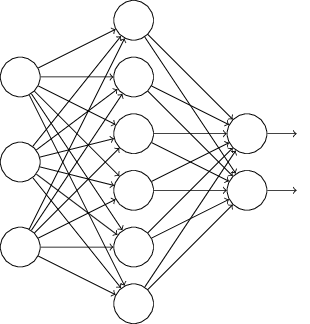
\includegraphics[width=4cm]{Sources/Figures/fully_connected_layer.png}
    \caption{Multilayer Perceptron with two fully-connected layers. Taken from \cite{nielsenneural}.}
    \label{fig:fcl}
\end{figure}

\subsection{Convolution Layer}
The most important layer of CNNs is the \textbf{convolution layer}. It introduces a new concept of shared weights, which help us train deeper architectures and is more suited for image processing tasks. To illustrate the convolution layer, imagine the input as a square of neurons, i.e., a two-dimensional \textbf{image} $\boldsymbol{I: (W, H) \rightarrow \real}$\todo{Zmatecna definice. Sjednotit styl notaci.}, where ${W}$ is the width and ${H}$ is the height of the image. 

In contrast with a fully-connected layer, we do not connect every input neuron to every output neuron. Instead, every output neuron is associated with a smaller region in the input image. Each association is defined by its \textbf{bias} $\boldsymbol{b}$ and $\textbf{weights}$ $\boldsymbol{K:(K_w, K_h) \rightarrow \real}$, where $K_w$, $K_h$ is the region's width and height. The output of the layer is a downscaled image $\boldsymbol{Y:(W - K_w + 1,}$ $\boldsymbol{H - K_h + 1)  \rightarrow \real}$, which is often called a \textbf{feature map}. The value of the $i, j$-th output neuron $Y(i,j)$ is defined by: 
$$
Y(i, j) = f\left((I * K)(i,j) + b\right)
$$

The $*$ operation is called \textbf{convolution}\todo{Fskutecnosti cross-correlation. Doplnit poznamku.} and is defined as follows:

$$
(I * K)(x, y) = \sum\limits_{k = 1}^{K_w}\sum\limits_{l = 1}^{K_h} I(x + k, y + l) \cdot K(k, l)
$$

This process is applied to the whole input image (see figure \ref{fig:convolution}). The convenience of this method comes with using the same weights $K$ for each convolution operation. The weights $K$ (and also bias $b$) are called \textbf{kernel} or \textbf{filter}. The kernel is trained to detect some non-linear pattern. Therefore, we use multiple kernels to recognize various features in the image (we end up with multiple feature maps). The approach also helps CNNs to adapt to image \textbf{translation invariance}, i.e., the detected features do not depend on their positions in the input image.

For illustration purpose, we have considered a two-dimensional inputs. However, in practice, we often work with RGB or even RGB-D images represented by \textbf{tensors} of shape $(W, H, C)$, where $C$ is number of channels (e.g. three for classic RGB image). 

Another important parameter of the layer is \textbf{stride length}. It defines the number of pixels the filters shifts over the input image. The bigger is stride length the more downscaled the output image is.


\begin{figure}[h]
    \centering
    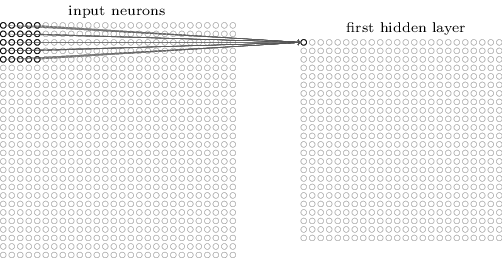
\includegraphics[width=10cm]{Sources/Figures/convolution.png}
    \caption{Illustration of a convolution layer with 5 $\times$ 5 kernel. Taken from \cite{nielsenneural}.}
    \label{fig:convolution}
\end{figure}

\subsection{Pooling Layer}
Another essential layer for CNNs is the \textbf{pooling layer}. In CNN architectures, the pooling layers typically come after the convolution layers. They are used for downscaling the feature maps to reduce the number of network parameters. 

The layer works in a similar manner to the convolution layer. It takes multiple values from a pooling region and outputs a single pixel. The most common type of a~ pooling operation is \textbf{max pooling}, which outputs the region's maximum value. Another operation that can be applied to the region is \textbf{average pooling}, which outputs the region's mean value.

The pooling region's shape is typically 2 $\times$ 2. In some cases, we want to pool from the whole input. We call these operations \textbf{global poolings} (e.g., global max pooling).

\subsection{Activation Functions}
\label{afunctions}

Activation functions introduce non-linearity to the layers. Some of the most important ones are listed below:
\begin{itemize}
\item \textbf{ReLU} (rectified linear unit) is the most popular activation function, which was introduced in \cite{pmlr-v15-glorot11a}. It is defined as follows: $\text{ReLU}(x) = \max(0, x)$. It deals better with vanishing gradient than sigmoidal functions, which tend to saturates on extreme values.
\item \textbf{Leaky ReLU} deals with the so-called \textbf{dying ReLU problem}. If we use simple ReLU, many neurons cannot recover from being stuck at zero value. We can tackle the problem by "leaking out" the negative values. The leaked values are then weighted by parameter $\alpha$: $\text{Leaky ReLU}(x) = \max(\alpha x, x)$
\item \textbf{Softmax} funciton is typically used in a last layer of classification neural networks. It takes a vector of real numbers and normalizes the values into a probability distribution. For input vector $x \in \real^K$ and output vector $y \in \real^K$, the function is defined as follows:
$$
    y_i = \text{softmax}(x)_i = \frac{e^{x_i}}{\sum\limits^{K}_{j = 1} e^{x_j}} \text{ for } i = 1,...,K
$$
\end{itemize}

\section{Training}
\begin{itemize}
    \item Optimization task
    \item Gradient descent
    \item Backpropagation
    \item Adam, etc.
\end{itemize}

\section{Overfitting and underfitting}

When we train a machine learning model, we typically have a \textbf{training set} and a \textbf{test set}. We then fit the model's parameters on a training set to \textbf{minimize} an error measure (a \textbf{training loss} or \textbf{error}). However, at the same time, we want to minimize a \textbf{test error} as well. We say that a model should \textbf{generalize}. This means that it should perform well on unseen data.

These efforts can lead to two major problems in machine learning. If we train for too long, the model will learn the training set patterns that do not generalize to the test set. We say that the model \textbf{overfits}. The opposite of overfitting is \textbf{underfitting}. It occurs when the model is not able to gain sufficiently low training loss. Underfitting can happen because of using a weak model or not training long enough. If we plot the losses, we want to make sure that the training loss is reasonably low, and the gap between training and test error is small (see figure \ref{fig:loss_plot}).
 
\begin{figure}[h]
    \centering
    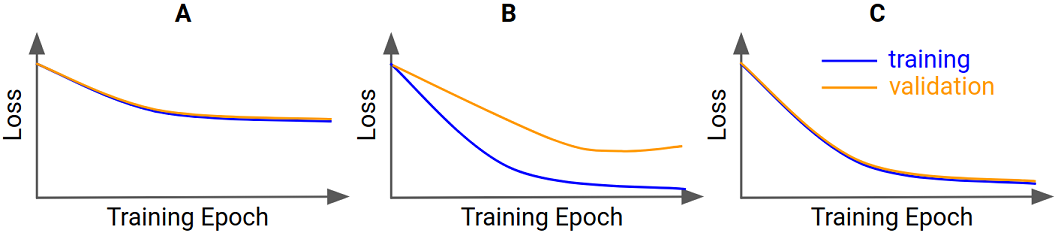
\includegraphics[width=\linewidth]{Sources/Figures/fitting.png}
    \caption{A simplified cases of loss curves \protect\footnotemark showing: (A) Underfitting, (B) Overfitting and (C) Optimal fit. Taken from \cite{bileschi2020deep}.}
    \label{fig:loss_plot}
\end{figure}

\footnotetext{The terms validation and test set are sometimes used interchangeably. However, the true meaning is not important for the illustration. Both are unobserved data.}

In coming subsections we describe the most common techniques to prevent overfitting in neural networks.
\footnotetext[2]{The simplest explanation is most likely the right one.}
\subsection{$L_2$ Regularization}
Following the Occam's razor principle\footnotemark , the extreme weights are likely to cause overfitting. We can reduce the overfitting by penalizing these weights with $\boldsymbol{L_2}$ \textbf{regularization}. The penalization is performed by adding a $L_2$ term to the loss function. The term is defined as a sum of squares of weight values. 



\subsection{Dropout}
Another common technique is called \textbf{dropout}. This method prevents individual nodes in the network to rely on the output of other nodes by randomly "dropping out" or "deactivating" some of the neurons. The method's parameter is a number between 0 and 1 that defines the fraction of the input units to drop.

\subsection{Batch Normalization}
Deep neural networks often suffer from unstability. Small changes in layers close to the input amplify as they propagate through the network. The deeper layers have to adapt significantly and thus learn slowly. \textbf{Batch normalization} introduces a way to stabilize and accelerate the training speed by normalizing the outputs of previous layer by subtracting the batch mean and dividing by the batch standard deviation.

\subsection{Data Augmentation}
The most obvious way to train a robust model is to have an extensive dataset. However, in some cases, it is very challenging to acquire sufficient ammount of data. We can overcome this issue by 
\textbf{augmenting} the training set by generating new artificial data. Of course, it is impossible to adopt this approach to every type of datasets, but it is straightforward for object detection tasks. The simplest way to augment the image dataset is by adding \textbf{random transformations} (cropping, resizing, rotation, ...) of the original images. The more sophisticated method would be generating new \textbf{synthetic} images. With recent advances in generative adversarial networks (GANs), it is possible to synthesize high-quality images. An impressive adoption of this approach is proposed in \cite{wei2019generative}.



  %%%%%%%%%%%%%%%%%%%%%%%%%%%%%%%%%%%%%%%%%%%%%%%%%%%%%%%%%%%%%%%%%%%%%%%%
\chapter{Object Detection}
%%%%%%%%%%%%%%%%%%%%%%%%%%%%%%%%%%%%%%%%%%%%%%%%%%%%%%%%%%%%%%%%%%%%%%%%
\textcolor{red}{(Sloučit s úvodem?)}

Object detection aims to locate objects in a given image and assign them to their class (also called category or label). The task can be broken down into three steps: informative region selection, feature extraction, and classification. In the first step, the method has to determine regions to which we apply the feature extraction. The extracted semantic representation for each selected region is then used to predict the target's class. 

Traditionally, engineers had to hand-craft feature extractors using algorithms such as SIFT \cite{sift}, SURF \cite{surf}, or HOG \cite{hog}. These methods are combined with well-established classification algorithms such as Support Vector Machines (SVM) \cite{svm}. Since this approach needs manual designing, it can be very demanding.

Deep learning methods introduced an end-to-end learning approach, which means that the model only takes a given set of annotated images to learn to detect key features, localize the objects, and classify them. So the hard work is done mainly by the model itself. This approach outperforms the traditional pipelines by a significant margin with respect to illumination and viewpoint changes \cite{outperforming}. For illustrative comparison see Figure \ref{fig:comparison}. We describe deep learning in detail in the following Chapter \ref{deep_learning_chapter}.

\begin{figure}[h]
    \centering
    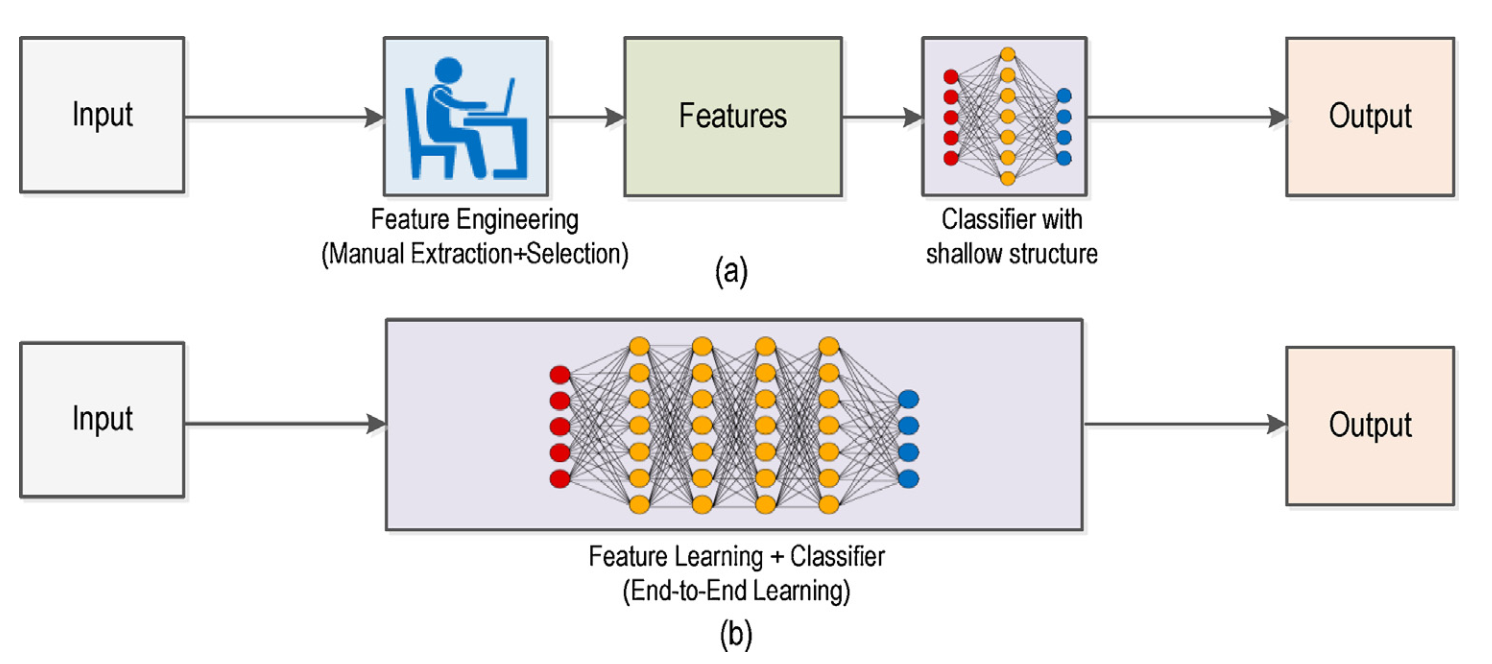
\includegraphics[width=\linewidth]{Sources/Figures/comparison.png}
    \caption{Comparison of: (a) Traditional approach and (b) Deep learning approach. Adapted from \cite{comparison_illustration}. \todo{Zmenit obrazek, clovek mate.}}
    \label{fig:comparison}
\end{figure}



% This ensures that the subsequent sections are being included as root
% items in the bookmark structure of your PDF reader.
\bookmarksetup{startatroot}
\backmatter

  \begingroup
    \let\clearpage\relax
    \glsaddall
    \printglossary[type=\acronymtype]
    \newpage
    \printglossary
  \endgroup

  \printindex
  \printbibliography

\end{document}
